\documentclass[conference, a4paper]{IEEEtran}

\usepackage{cite}
\usepackage{amsmath,amssymb,amsfonts}
\usepackage{algorithmic}
\usepackage{graphicx}
\usepackage{textcomp}
\usepackage{xcolor}
\usepackage{hyperref} % Para enlaces y referencias cruzadas
\usepackage{fancyhdr} % Para controlar los encabezados y pies de página
\usepackage{float} % Para usar el modificador H en figuras

% Agregar números de página
\pagestyle{plain}

\begin{document}

\title{Práctica 1: Programa MPI simple y caracterización del rendimiento}
\author{
    \IEEEauthorblockN{Jorge Otero y Pablo Seijo}
    \IEEEauthorblockA{Fundamentos de Sistemas Paralelos\\
    Universidad de Santiago de Compostela\\
    Email: pablo.garcia.seijo@rai.usc.es }
}
\date{\today}

\maketitle

\begin{abstract}
En esta práctica se aborda la implementación y el análisis de un programa paralelo con MPI para calcular el valor de \(\pi\) mediante el método de Monte Carlo. Se evaluó el rendimiento en términos de tiempo de ejecución, eficiencia y calidad de los resultados al variar el número de procesos y el número de iteraciones. Los experimentos demuestran que el método es escalable y que la eficiencia mejora conforme aumenta el tamaño del problema.
\end{abstract}

% Agregar las palabras clave
\begin{IEEEkeywords}
MPI, Monte Carlo, paralelismo, eficiencia, speed-up, escalabilidad.
\end{IEEEkeywords}

\section{Introducción}
El cálculo de \(\pi\) ha sido objeto de estudio en numerosos contextos computacionales, especialmente por su importancia en pruebas de rendimiento de algoritmos paralelos. En esta práctica, se implementa un programa en C utilizando MPI para paralelizar el cálculo de \(\pi\) mediante el método de Monte Carlo. Se analizan el tiempo de ejecución, la eficiencia y la calidad de los resultados, que se mide como la inversa del producto entre el tiempo y el error.

\section{Metodología}
La implementación se realizó en C utilizando MPI para gestionar la comunicación entre procesos. El método de Monte Carlo para el cálculo de \(\pi\) se basa en la generación de puntos aleatorios y la evaluación de cuántos de ellos caen debajo de la curva definida por una función relacionada con \(\pi\). El programa divide el número total de iteraciones entre los procesos y utiliza una estrategia de reducción en árbol binario para recopilar y combinar los resultados parciales.

El tiempo de ejecución se mide utilizando \texttt{MPI\_Wtime()}, y la eficiencia se calcula como el cociente entre el speed-up y el número de procesos:

\begin{equation}
\text{Eficiencia} = \frac{S}{P}
\end{equation}

donde \( S \) es el speed-up, definido como:

\begin{equation}
S = \frac{T_{\text{secuencial}}}{T_{\text{paralelo}}}
\end{equation}

y \( P \) es el número de procesos.

\section{Resultados}
Los resultados se presentan en forma de gráficos que ilustran el comportamiento del programa en términos de eficiencia, speed-up, calidad del resultado y error.

\subsection{Eficiencia vs Número de Iteraciones}
\begin{figure}[h!]
    \centering
    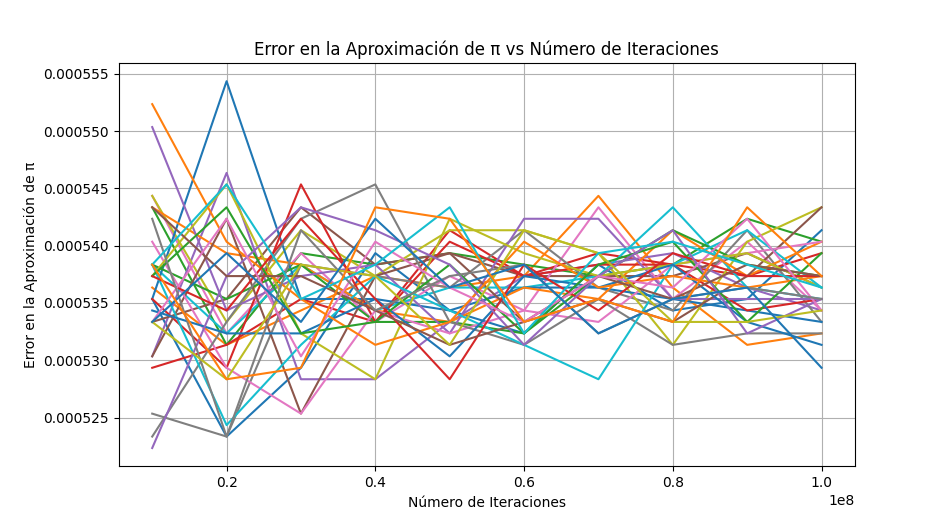
\includegraphics[width=0.45\textwidth]{Figure_1.png}
    \caption{Eficiencia en función del número de iteraciones.}
    \label{fig:eficiencia}
\end{figure}
El gráfico muestra que la eficiencia mejora a medida que aumenta el número de iteraciones, acercándose al valor óptimo de 1 en configuraciones de mayor tamaño de problema.

\subsection{Speed-up vs Número de Iteraciones}
\begin{figure}[h!]
    \centering
    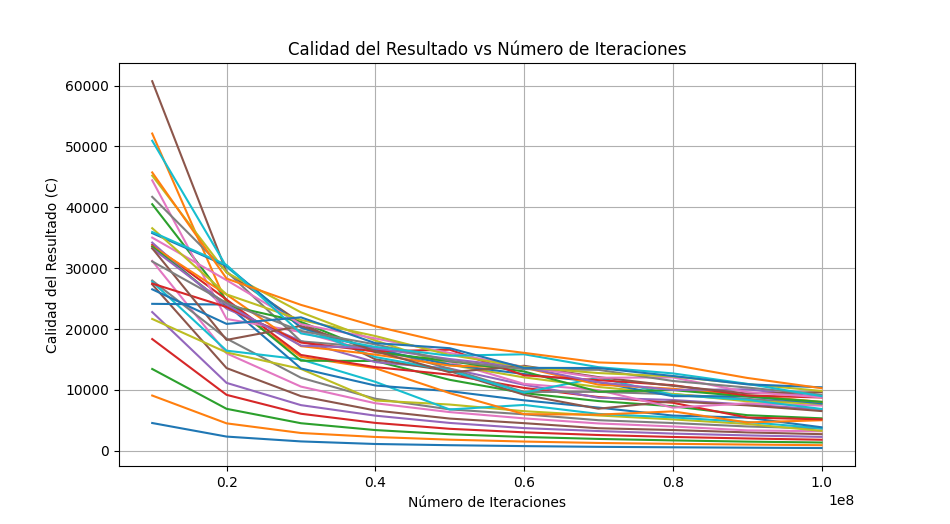
\includegraphics[width=0.45\textwidth]{Figure_2.png}
    \caption{Speed-up en función del número de iteraciones.}
    \label{fig:speedup}
\end{figure}
Se observa que el speed-up aumenta con el número de iteraciones, lo que indica un uso eficiente de los recursos de cálculo.

\subsection{Calidad del Resultado vs Número de Iteraciones}
\begin{figure}[h!]
    \centering
    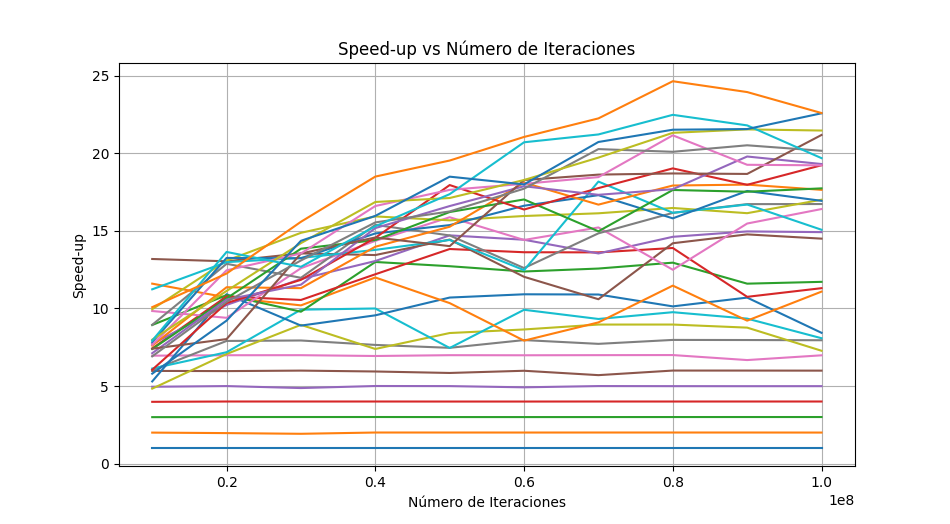
\includegraphics[width=0.45\textwidth]{Figure_3.png}
    \caption{Calidad del resultado en función del número de iteraciones.}
    \label{fig:calidad}
\end{figure}
La calidad del resultado mejora con el aumento del número de iteraciones, mostrando una reducción en el error relativo y tiempos de ejecución más cortos.

\subsection{Error en la Aproximación de \(\pi\)}
\begin{figure}[h!]
    \centering
    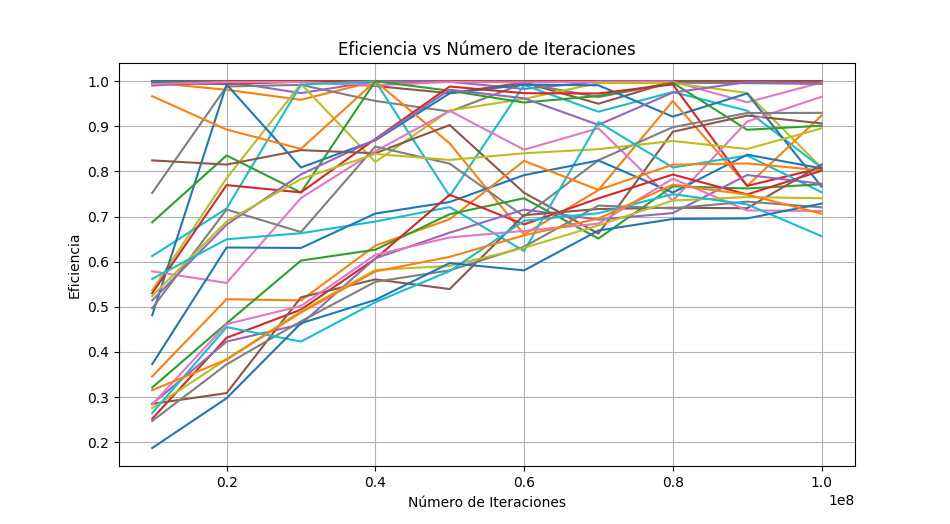
\includegraphics[width=0.45\textwidth]{Figure_4.png}
    \caption{Error en la aproximación de \(\pi\) en función del número de iteraciones.}
    \label{fig:error}
\end{figure}
El error en la aproximación tiende a estabilizarse conforme aumenta el número de iteraciones, lo que demuestra la efectividad del método.

\section{Conclusiones}
El programa implementado para el cálculo de \(\pi\) mediante el método de Monte Carlo, distribuido con MPI, demuestra una mejora en la eficiencia y la calidad del resultado al incrementar el número de iteraciones. La estrategia de reducción en árbol binario permite una recopilación eficiente de los datos parciales, y el uso de MPI garantiza una buena escalabilidad.


\bibliographystyle{IEEEtran}
\bibliography{bibliografia}

\end{document}